\documentclass[13pt, aspectratio=169]{beamer}
\usepackage[utf8]{inputenc} 
\usepackage{caption} 
\usepackage[spanish]{babel} 
\usepackage{graphicx} % Required for inserting images
\usepackage{tikz}
\usepackage{svg}
\usepackage{amsfonts} 
\usepackage{amsmath}
\usepackage{bm}
\usepackage{amssymb} 
\usepackage{lipsum} % texto predeterminado
\usepackage{ragged2e} % para justificar texto
\usepackage[backend=biber, style=authoryear]{biblatex}
\addbibresource{Referencias.bib}
\AtBeginBibliography{\small}

\usepackage{svrsymbols} % para poner particulas como electrones, mesones, etc
\usepackage{mhchem} % poner compuestos quimicos e isotopos
\usepackage{chemfig}

\usepackage{siunitx}

% \captionsetup{labelformat=empty} % para quitar el caption.

% Muestra el número de la diapositiva
\setbeamertemplate{footline}[frame number]

%---- Definimos colores -----
\usepackage{xcolor}    % Necesario para definir colores personalizados en RGB
\usepackage{tcolorbox} % Necesario para crear cuadros con bordes redondeados
\definecolor{azul}{rgb}{0.17, 0.40, 0.69} % color que quiero en rgb
\setbeamercolor{structure}{fg=azul} % lo definimos para todo el beamer

% Define los colores del bloque
\definecolor{custombgcolor2}{RGB}{201, 123, 219} % Color de fondo
\definecolor{custombgcolor3}{RGB}{231, 185, 104} % Color de fondo
\definecolor{custombgcolor4}{RGB}{91, 185, 178} % Color de fondo
\definecolor{custombgcolor5}{RGB}{228, 220, 88} % Color de fondo
\definecolor{custombgcolor6}{RGB}{78, 157, 116} % Color de fondo
\definecolor{custombgcolor7}{RGB}{81, 183, 224} % Color de fondo
\definecolor{custombgcolor8}{RGB}{150, 161, 166} % Color de fondo
\definecolor{custombgcolor9}{RGB}{69, 247, 146} % Color de fondo

\definecolor{customfgcolor1}{RGB}{255, 255, 255} % Color del texto
\definecolor{customfgcolor2}{RGB}{0, 0, 0} % Color del texto

\usetheme{Rochester} % tema para usar en este slide

%--------------- Para que se ponga la lista de contenido mas interesante
\AtBeginSection[]
{
    \begin{frame}<beamer>{Contenido}
        \tableofcontents[currentsection, currentsubsection]
    \end{frame}
}
\AtBeginSubsection[]
{
    \begin{frame}<beamer>{Contenido}
        \tableofcontents[currentsection, currentsubsection]
    \end{frame}
}

%-------------------------- Quitar el menu de la lateral inferior izquierda
\setbeamertemplate{navigation symbols}{}

%--------------------------------------------

\title{\Large Estudio de la variación con la altura del flujo atmosférico de protones y neutrones secundarios producidos por rayos cósmicos}
\author{Presenta: Mata \\ 
    \scriptsize Director de tesis: Dr. Oscar Gustavo Morales Olivares}
\institute{
    \inst{
        \footnotesize Universidad Nacional Autónoma de México 
    }
    \inst{
        \footnotesize Facultad de Ciencias
    }
}
\date{\scriptsize x de octubre de 2024}

\begin{document}

\begin{frame}[plain]
    \begin{minipage}[t]{0.1\linewidth}
        \includegraphics[width=2cm]{Figures/unam.pdf}
    \end{minipage}
    \hfill
    \begin{minipage}[t]{0.1\linewidth}
        \includegraphics[width=2cm]{Figures/ciencias.pdf}
    \end{minipage}
    \vspace{2cm}
    \titlepage
\end{frame}


%--------------------------------------------

    %\begin{frame} % cada entorno frame es una diapositiva
        %\maketitle
    %\end{frame}
    
    \begin{frame}{Contenido} % cada entorno frame es una diapositiva
        \tableofcontents
    \end{frame}
    
	%----------- SLIDES -------------
	%---------------------------------------------------------------------   
    \section{Introducción}
    %------------------------------ SLIDE ---------------------------------------
    \setbeamertemplate{itemize item}{\raisebox{0.2ex}{\scriptsize$\blacktriangleright$}}
    \setbeamercolor{itemize item}{fg=red} % Cambia el color del triángulo a naranja    
    \begin{frame}{Introducción} % cada entorno frame es una diapositiva
        \justifying % para justificar el texto, siempre al inicio de cada frame
        % Añade espacio para mover el bloque hacia arriba
        % Añade espacio para mover el bloque hacia arriba
        \vspace*{-0.6cm} % Ajusta este valor según sea necesario
        
        % Define los colores del bloque
        %\definecolor{custombgcolor2}{RGB}{201, 123, 219} % Color de fondo
        %\definecolor{customfgcolor2}{RGB}{0, 0, 0} % Color del texto

        % Cuadro sin bordes redondeados, con colores personalizados
        \begin{tcolorbox}[colback=custombgcolor2, coltext=customfgcolor2,
                      colframe=custombgcolor2, % Color del borde
                      width=\textwidth,       % Ancho del cuadro
                      boxrule=1pt,            % Grosor del borde
                      top=1mm, bottom=1mm,     % Espacio superior e inferior
                      sharp corners=all,     % Bordes sin redondear
                      halign=center,         % Alineación horizontal
                      valign=center,         % Alineación vertical
                      ]
            % Texto dentro del cuadro
            % \textbf{Rayos \kern-0.9em Cósmicos \kern-0.9em (RC)}
            \textbf{¿Qué \kern-0.9em son \kern-0.9em los \kern-0.9em Rayos \kern-0.9em Cósmicos?}
        \end{tcolorbox}

        \begin{columns}
            \begin{column}{0.7\textwidth} % Columna izquierda para la lista
                \begin{itemize}
                    \item Núcleos de átomos desprovistos de sus electrones. 
                    \item Consisten en $\sim 90\%$ protones, $\sim 9\%$ núcleos de helio y $\sim 1\%$ otros núcleos más pesados.
                    \item Llegan a la Tierra desde todas direcciones.
                    \item Descubiertos por \emph{Victor Hess} en 1912.
                \end{itemize}
            \end{column}

            \begin{column}{0.3\textwidth} % Columna derecha para la imagen
                \begin{figure}
                    \centering
                    \includegraphics[width=0.5\textwidth]{Figures/vhess.jpg}
                    \caption{\tiny Victor Hess recibió el premio Nobel de Física en 1936 por su descubrimiento de los rayos cósmicos.}
                \end{figure}
            \end{column}            
        \end{columns} 
    \end{frame}

    %------------------------------ SLIDE --------------------------------------- SLIDE DE PRUEBA ESPECTRO DE ENERGIA + METODOS DE DETECCION
    \begin{frame}{} % cada entorno frame es una diapositiva
        \justifying % para justificar el texto, siempre al inicio de cada frame
        % Añade espacio para mover el bloque hacia arriba
        % Añade espacio para mover el bloque hacia arriba
        \vspace*{-1.55cm} % Ajusta este valor según sea necesario
        
        % Define los colores del bloque
        %\definecolor{custombgcolor3}{RGB}{231, 185, 104} % Color de fondo
        %\definecolor{customfgcolor2}{RGB}{0, 0, 0} % Color del texto

        % Cuadro sin bordes redondeados, con colores personalizados
        \begin{tcolorbox}[colback=custombgcolor3, coltext=customfgcolor2,
                      colframe=custombgcolor3, % Color del borde
                      width=\textwidth,       % Ancho del cuadro
                      boxrule=1pt,            % Grosor del borde
                      top=1mm, bottom=1mm,     % Espacio superior e inferior
                      sharp corners=all,     % Bordes sin redondear
                      halign=center,         % Alineación horizontal
                      valign=center,         % Alineación vertical
                      ]
            % Texto dentro del cuadro
            \textbf{Espectro \kern-0.9em de \kern-0.9em Energía}
        \end{tcolorbox}

        \begin{columns}
            \begin{column}{0.5\textwidth} % Columna izquierda para la lista
                \begin{itemize}
                    \item Ley de potencia: $\bm{\Phi}\mathbf{(E) \propto E}^{\bm{-\alpha}}$,
                    
                    donde $\mathbf{E}$ es la energía y $\bm{\alpha}$ el índice espectral.
                    \item Abarca varios ordenes de magnitud ($\sim \bm{10^{8}}$ a $\sim \bm{10^{21}}$) \textbf{eV}.
                    \item Son muy abundantes los rayos cósmicos de \textbf{baja energía}.
                    \item Los rayos cósmicos pueden ser detectados de manera \textbf{directa} e \textbf{indirecta}.
                    %\item Índice espectral $\bm{\alpha}$.
                    %\item La \textbf{rodilla} es donde se produce un cambio en el valor de $\bm{\alpha}$.
                    %\item En la región del \textbf{tobillo} el valor del índice cambia $\bm{\alpha} \mathbf{\sim 2}$.\textbf{6}.
                \end{itemize}
            \end{column}

            \begin{column}{0.4\textwidth} % Columna derecha para la imagen
                \begin{figure}
                    \centering
                    \includegraphics[width=1.0\textwidth]{Figures/spectrum2.png}
                    \caption{\tiny Espectro de los RC, se muestra los instrumentos usados para la detección a diferentes altitudes. Imagen tomada del \href{https://revista.iaa.csic.es/content/portada/404/69}{Instituto de Astrofísica de Andalucía (IAA-CSIC)} (2023).}                    
                \end{figure}
            \end{column}
        \end{columns}
    \end{frame}

    %------------------------------ SLIDE --------------------------------------- SLIDE ORIGINAL ESPECTRO DE ENERGIA
    %\begin{frame}{} % cada entorno frame es una diapositiva
        %\justifying % para justificar el texto, siempre al inicio de cada frame
        % Añade espacio para mover el bloque hacia arriba
        % Añade espacio para mover el bloque hacia arriba
        %\vspace*{-1.55cm} % Ajusta este valor según sea necesario
        
        % Define los colores del bloque
        %\definecolor{custombgcolor3}{RGB}{231, 185, 104} % Color de fondo
        %\definecolor{customfgcolor2}{RGB}{0, 0, 0} % Color del texto

        % Cuadro sin bordes redondeados, con colores personalizados
        %\begin{tcolorbox}[colback=custombgcolor3, coltext=customfgcolor2,
                      %colframe=custombgcolor3, % Color del borde
                      %width=\textwidth,       % Ancho del cuadro
                      %boxrule=1pt,            % Grosor del borde
                      %top=1mm, bottom=1mm,     % Espacio superior e inferior
                      %sharp corners=all,     % Bordes sin redondear
                      %halign=center,         % Alineación horizontal
                      %valign=center,         % Alineación vertical
                      %]
            % Texto dentro del cuadro
            %\textbf{Espectro \kern-0.9em de \kern-0.9em Energía}
        %\end{tcolorbox}

        %\begin{columns}
            %\begin{column}{0.45\textwidth} % Columna izquierda para la lista
                %\begin{itemize}
                    %\item Ley de potencia: $\bm{\Phi}\mathbf{(E) \propto E}^{\bm{-\alpha}}$.
                    %\item La región donde el índice espectral $\bm{\alpha} \mathbf{\sim 2}$.\textbf{7} podrían provenir de nuestra galaxia.
                    %\item La \textbf{rodilla} es donde se produce un cambio en el valor de $\bm{\alpha}$.
                    %\item En la región del \textbf{tobillo} el valor del índice cambia $\bm{\alpha} \mathbf{\sim 2}$.\textbf{6}.
                %\end{itemize}
            %\end{column}

            %\begin{column}{0.4\textwidth} % Columna derecha para la imagen
                %\begin{figure}
                    %\centering
                    %\includegraphics[width=1.0\textwidth]{Figures/spectrum.png}
                    %\caption{\tiny Espectro de energía de los RC [\cite{evoli2018}].}                    
                %\end{figure}
            %\end{column}
        %\end{columns}
    %\end{frame}
    
    %------------------------------ SLIDE --------------------------------------- SLIDE ORIGINAL DE ORIGEN DE RC
    %\begin{frame}{} % cada entorno frame es una diapositiva
        %\justifying % para justificar el texto, siempre al inicio de cada frame
        % Añade espacio para mover el bloque hacia arriba
        % Añade espacio para mover el bloque hacia arriba
        %\vspace*{-0.4cm} % Ajusta este valor según sea necesario

        % Cuadro sin bordes redondeados, con colores personalizados
        %\begin{tcolorbox}[colback=custombgcolor2, coltext=customfgcolor2,
                      %colframe=custombgcolor2, % Color del borde
                      %width=\textwidth,       % Ancho del cuadro
                      %boxrule=1pt,            % Grosor del borde
                      %top=1mm, bottom=1mm,     % Espacio superior e inferior
                      %sharp corners=all,     % Bordes sin redondear
                      %halign=center,         % Alineación horizontal
                      %valign=center,         % Alineación vertical
                      %]
            % Texto dentro del cuadro
            %\textbf{Origen \kern-0.9em de \kern-0.9em los \kern-0.9em Rayos \kern-0.9em Cósmicos}
        %\end{tcolorbox}
        
        %\begin{figure}
        	%\centering
        	%\includegraphics[width=0.5\textwidth]{Figures/sourcestable1.png}
        	%\caption{\tiny Posibles fuentes de rayos cósmicos [\cite{spurio2018}].} 
        %\end{figure}
    %\end{frame}  

    %------------------------------ SLIDE --------------------------------------- SLIDE DE PRUEBA DE ORIGEN DE RC
    \begin{frame}{} % cada entorno frame es una diapositiva
        \justifying % para justificar el texto, siempre al inicio de cada frame
        % Añade espacio para mover el bloque hacia arriba
        % Añade espacio para mover el bloque hacia arriba
        \vspace*{-1.6cm} % Ajusta este valor según sea necesario
        % Cuadro sin bordes redondeados, con colores personalizados
        \begin{tcolorbox}[colback=custombgcolor2, coltext=customfgcolor2,
                      colframe=custombgcolor2, % Color del borde
                      width=\textwidth,       % Ancho del cuadro
                      boxrule=1pt,            % Grosor del borde
                      top=1mm, bottom=1mm,     % Espacio superior e inferior
                      sharp corners=all,     % Bordes sin redondear
                      halign=center,         % Alineación horizontal
                      valign=center,         % Alineación vertical
                      ]
            % Texto dentro del cuadro
            \textbf{Origen \kern-0.9em de \kern-0.9em los \kern-0.9em Rayos \kern-0.9em Cósmicos}
        \end{tcolorbox}

        \vspace*{0.5cm} % Ajusta este valor según sea necesario
        
        \begin{columns}
            \begin{column}{0.5\textwidth}
                \centering
                \fcolorbox{black}{custombgcolor5}{
                    \parbox[c][0.5cm][c]{0.8\textwidth}{
                        \centering
                        Galáctico
                    }
                }

                \vspace*{0.5cm} % Ajusta este valor según sea necesario
                \begin{figure}
                    \centering
				    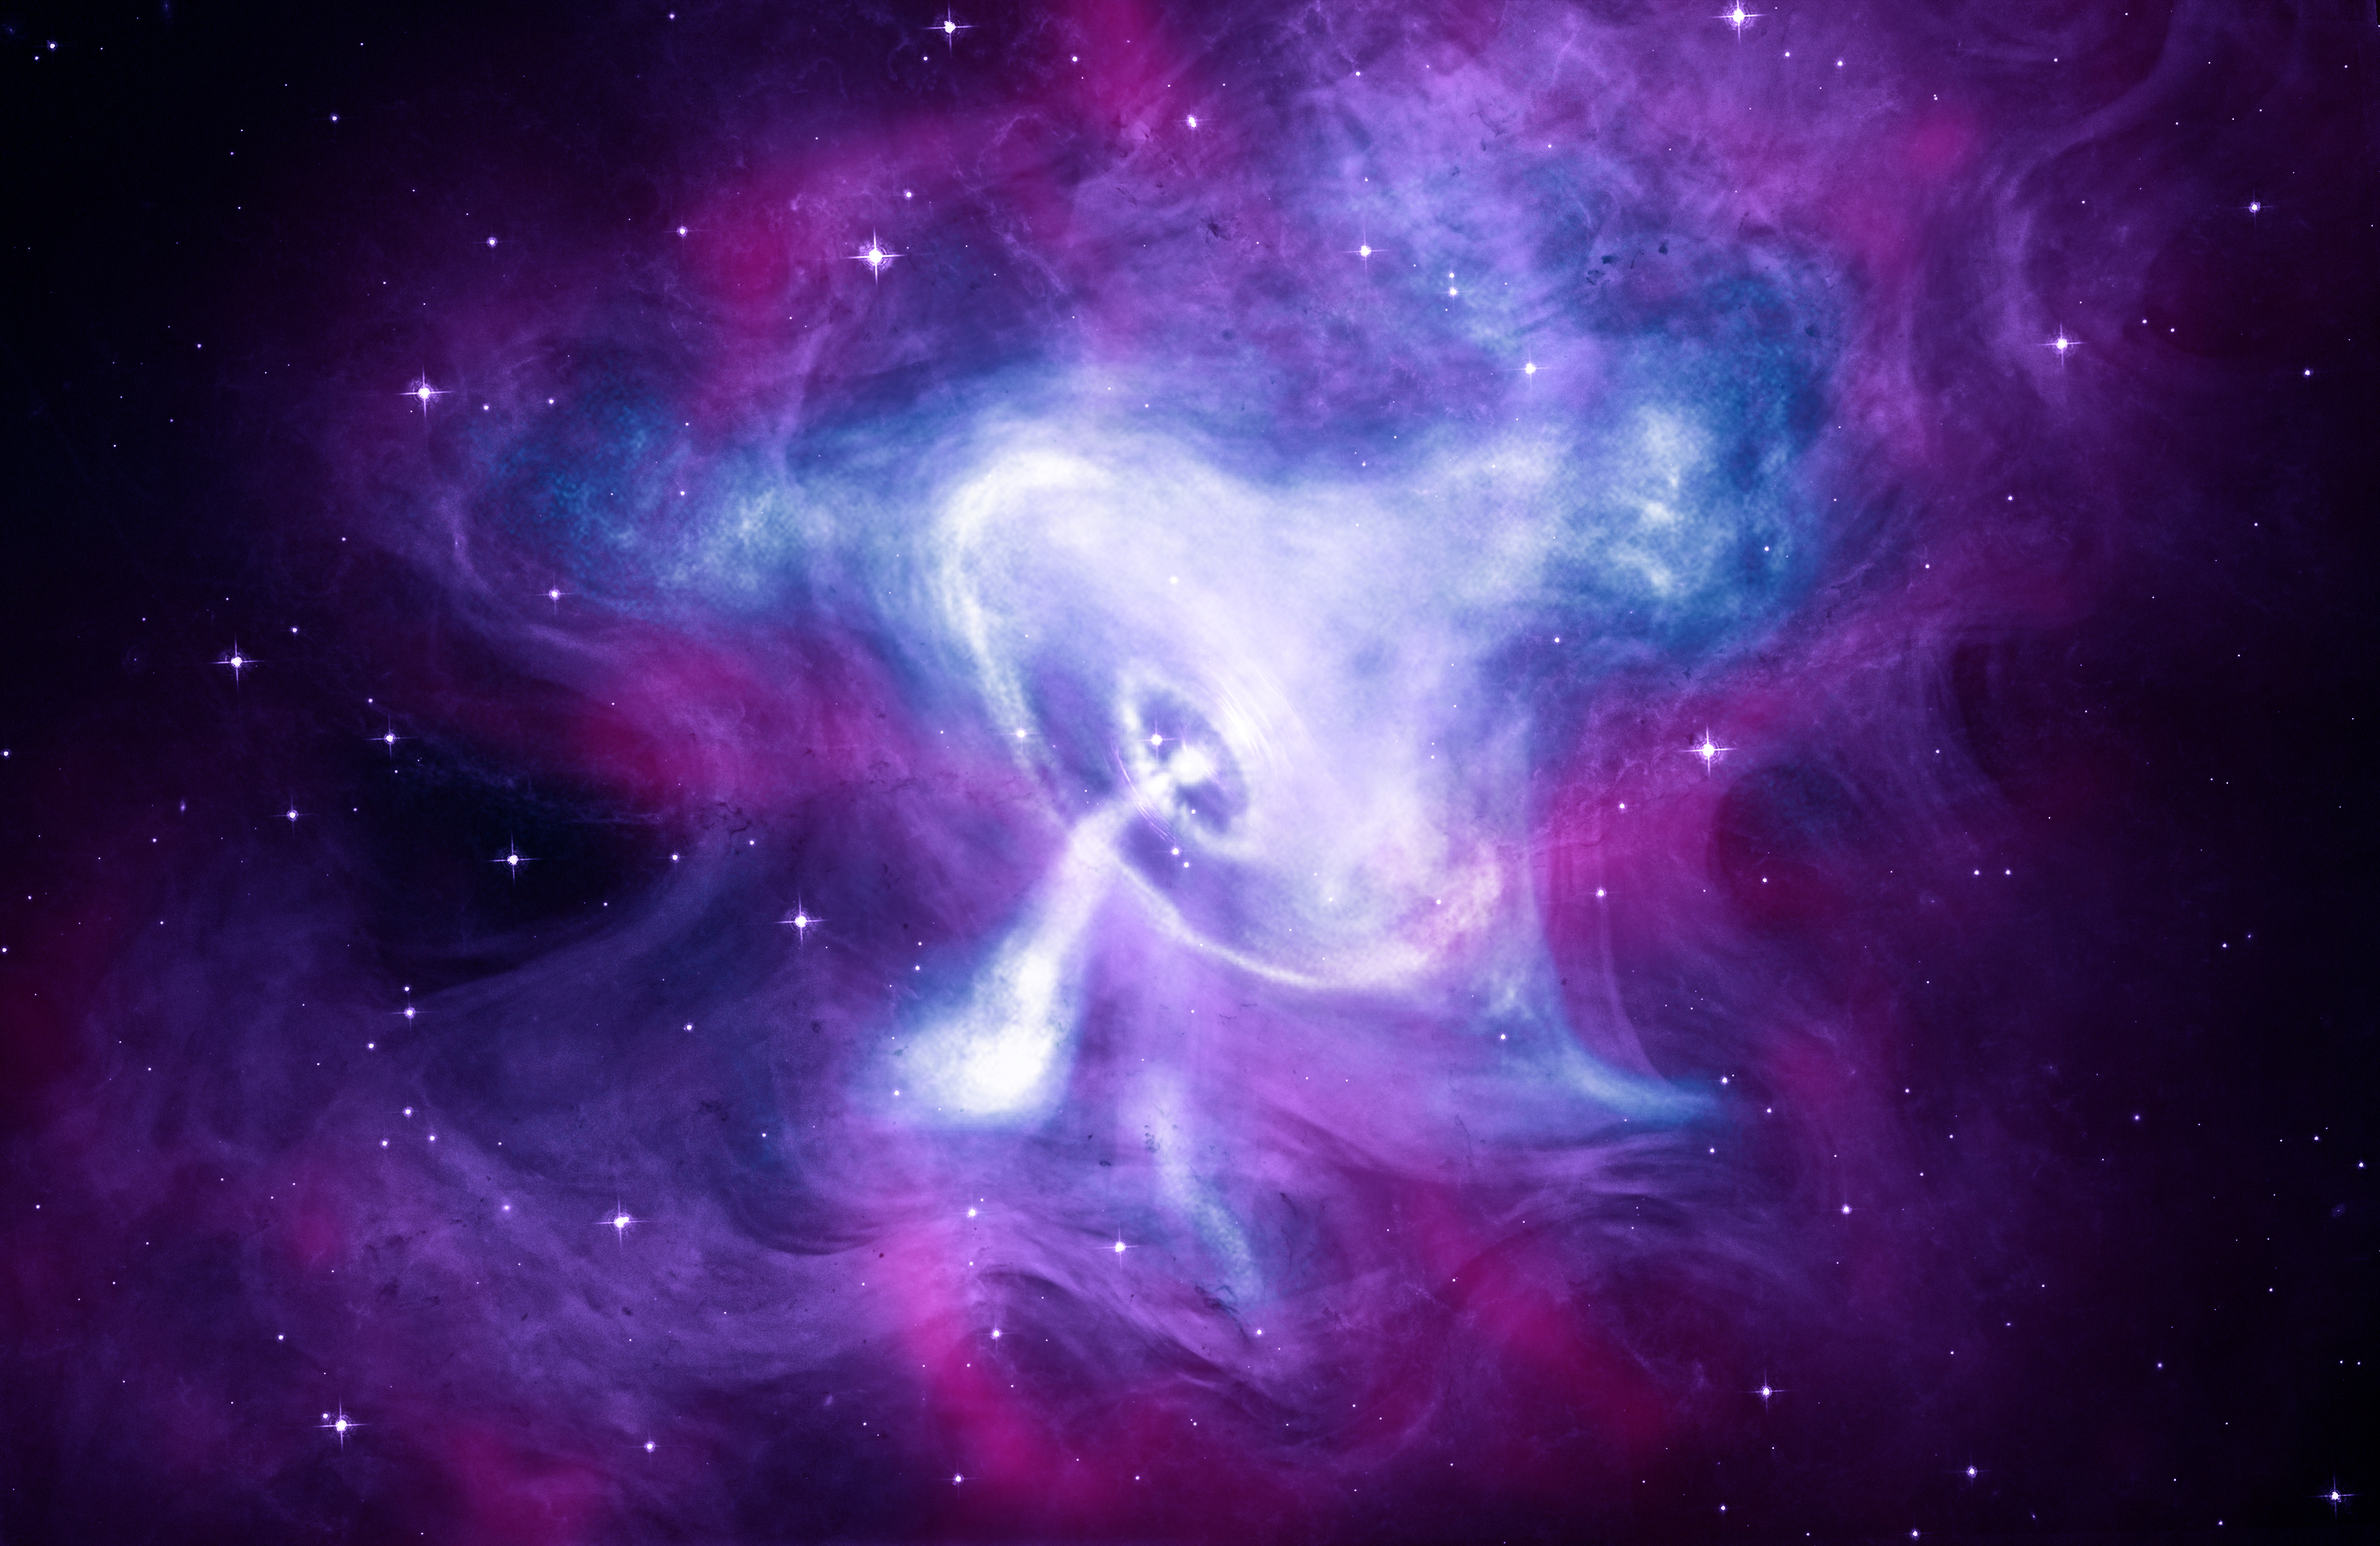
\includegraphics[width=0.9\textwidth]{Figures/remanetsupernova1.jpg}
				    \caption{\tiny Remanente de supernova en la \textbf{nebulosa del Cangrejo}, se encuentra a $6500$ años luz de la Tierra. Créditos: Rayos X: NASA/CXC/SAO; Visible: NASA/STScI; Infrarrojo: NASA-JPL-Caltech.}
                \end{figure}
                
            \end{column}

            \begin{column}{0.5\textwidth}
                \centering
                \fcolorbox{black}{custombgcolor7}{
                    \parbox[c][0.5cm][c]{0.8\textwidth}{
                        \centering
                        Extragaláctico
                    }
                }

                \vspace*{0.5cm} % Ajusta este valor según sea necesario
                \begin{figure}
                    \centering
				    \includegraphics[width=0.7\textwidth]{Figures/centaurusA_multiwavelength.png}
				    \caption{\tiny \textbf{Centaurus A} es una galaxia activa cercana a la Vía Láctea, ubicada a 3.5 megapársecs. Créditos: X-ray: NASA/CXC/SAO; optical: Rolf Olsen; infrared: NASA/JPL-Caltech; radio: NRAO/AUI/NSF/Univ.Hertfordshire/M.Hardcastle.}
                \end{figure}            
            \end{column}
        \end{columns}
    \end{frame}  

	%------------------------------ SLIDE --------------------------------------- SLIDE ORIGINAL DE ORIGEN DE RC
	%\begin{frame}{}
		%\begin{figure}
			%\centering
    		%\begin{minipage}{0.49\textwidth}
				%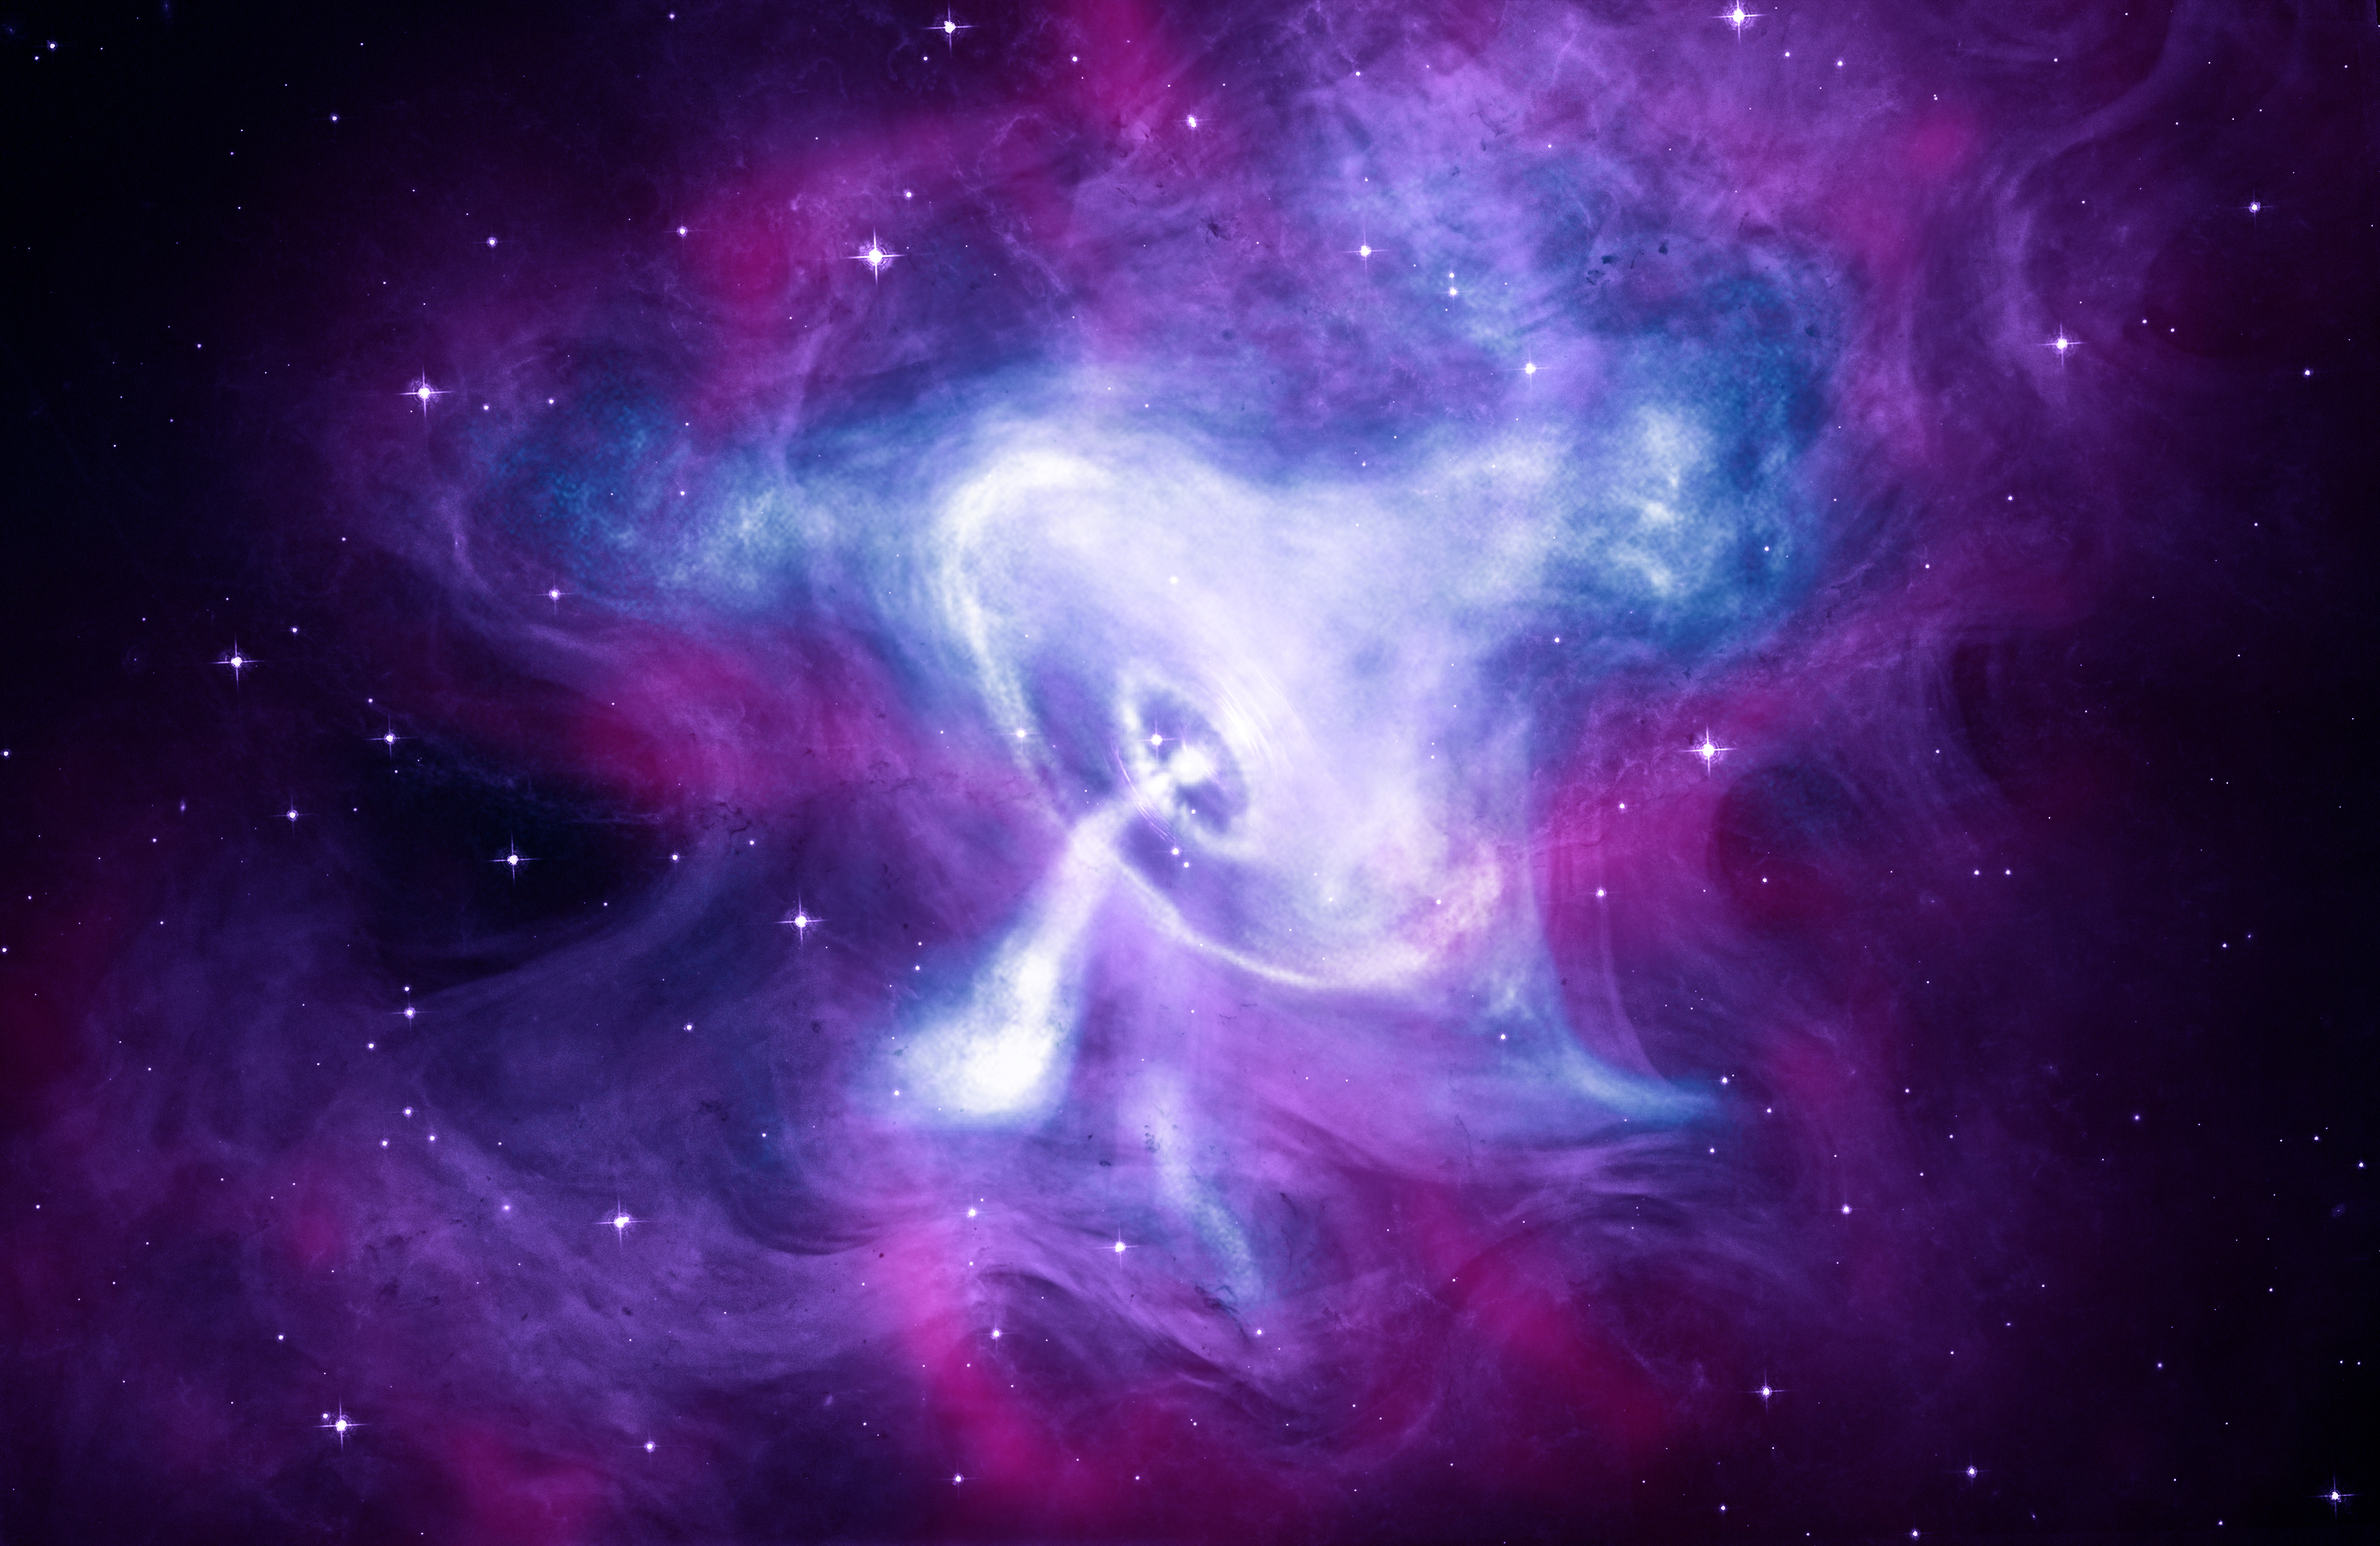
\includegraphics[width=\textwidth]{Figures/remanetsupernova1.jpg}
				%\caption{\tiny Remanente de supernova en la \textbf{nebulosa del Cangrejo}, se encuentra a $6500$ años luz de la Tierra. Créditos: Rayos X: NASA/CXC/SAO; Visible: NASA/STScI; Infrarrojo: NASA-JPL-Caltech.}
			%\end{minipage}
			%\hfill
			%\begin{minipage}{0.5\textwidth}
				%\includegraphics[width=\textwidth]{Figures/centaurusA_multiwavelength.png}
				%\caption{\tiny \textbf{Centaurus A} es una galaxia activa cercana a la Vía Láctea, ubicada a 3.5 megapársecs. Créditos: X-ray: NASA/CXC/SAO; optical: Rolf Olsen; infrared: NASA/JPL-Caltech; radio: NRAO/AUI/NSF/Univ.Hertfordshire/M.Hardcastle.}
			%\end{minipage}				
		%\end{figure}
	%\end{frame}

    %------------------------------ SLIDE ---------------------------------------
    \begin{frame}{} % cada entorno frame es una diapositiva
        \justifying % para justificar el texto, siempre al inicio de cada frame
        % Añade espacio para mover el bloque hacia arriba
        % Añade espacio para mover el bloque hacia arriba
        \vspace*{-0.5cm} % Ajusta este valor según sea necesario

        % Cuadro sin bordes redondeados, con colores personalizados
        \begin{tcolorbox}[colback=custombgcolor3, coltext=customfgcolor2,
                      colframe=custombgcolor3, % Color del borde
                      width=\textwidth,       % Ancho del cuadro
                      boxrule=1pt,            % Grosor del borde
                      top=1mm, bottom=1mm,     % Espacio superior e inferior
                      sharp corners=all,     % Bordes sin redondear
                      halign=center,         % Alineación horizontal
                      valign=center,         % Alineación vertical
                      ]
            % Texto dentro del cuadro
            \textbf{Rigidez \kern-0.9em umbral}
        \end{tcolorbox}

        \begin{columns}
            \begin{column}{0.45\textwidth} % Columna izquierda para la lista
                \begin{itemize}
                    \item Está dada por la ecuación: \[\mathbf{R} = \mathbf{\frac{pc}{Ze}},\]

                    donde $\mathbf{p}$ es el momento de la partícula, $\mathbf{c}$ es la velocidad de la luz, $\mathbf{Z}$ número de carga iónica  y $\mathbf{e}$ la carga elemental.
                    
                    \item Centro de México: $\mathbf{R_{c} \sim 8}$\textbf{.3 GV}.		
                \end{itemize}
            \end{column}
            
            \begin{column}{0.6\textwidth} % Columna derecha para la imagen
                \begin{figure}
                    \includegraphics[width=0.8\textwidth]{Figures/rigiditymap.png}
                    \caption{\tiny Mapa de la rigidez umbral de la Tierra [\cite{labrenz2014}].}
                \end{figure}
            \end{column}
        \end{columns}
    \end{frame}   

	%------------------------------ SLIDE ---------------------------------------
    \begin{frame}{} % cada entorno frame es una diapositiva
        \justifying % para justificar el texto, siempre al inicio de cada frame
        % Añade espacio para mover el bloque hacia arriba
        % Añade espacio para mover el bloque hacia arriba
        \vspace*{-0.2cm} % Ajusta este valor según sea necesario

        % Cuadro sin bordes redondeados, con colores personalizados
        \begin{tcolorbox}[colback=custombgcolor5, coltext=customfgcolor2,
                      colframe=custombgcolor5, % Color del borde
                      width=\textwidth,       % Ancho del cuadro
                      boxrule=1pt,            % Grosor del borde
                      top=1mm, bottom=1mm,     % Espacio superior e inferior
                      sharp corners=all,     % Bordes sin redondear
                      halign=center,         % Alineación horizontal
                      valign=center,         % Alineación vertical
                      ]
            % Texto dentro del cuadro
            \textbf{Cascada \kern-0.9em de \kern-0.9em partículas}
        \end{tcolorbox}

        \begin{columns}
            \begin{column}{0.57\textwidth} % Columna izquierda para la lista
                \begin{itemize}
                    \item \textcolor{blue}{\textbf{Componentes:}}
                    	\begin{itemize}
                    		\item Electromagnética.
                            \item Muónica.
                            \item Hadrónica.
                    	\end{itemize}
                    		
                    \item \textcolor{blue}{\textbf{Reacciones de decaimiento:}}
                    	\begin{itemize}
                            \item $\pionnull \rightarrow 2 \gamma$
                            \item $\pionplus \rightarrow \antimuon + \neutrino$
                            \item $\pionminus \rightarrow \muon + \antineutrino$
                    	\end{itemize}
                    \item \textcolor{blue}{\textbf{\small Vida media $\pionnull$:}} \small $\sim 10^{-16}$ s.
                    \item \textcolor{blue}{\textbf{\small Vida media de los piones ($\pionplus$ y $\pionminus$):}} \small $\sim 26$ ns.
                \end{itemize}
            \end{column}

            \begin{column}{0.3\textwidth} % Columna derecha para la imagen
                \begin{figure}
                    \centering
                    \includegraphics[width=0.88\textwidth]{Figures/showercomponent.png}
                    \caption{\tiny Esquema de las componentes de un chubasco de partículas [\cite{valdezgalicia1992}].}
                \end{figure}
            \end{column}
        \end{columns}
    \end{frame}     

    %------------------------------ SLIDE ---------------------------------------
    %\begin{frame}{} % cada entorno frame es una diapositiva
        %\justifying % para justificar el texto, siempre al inicio de cada frame
        % Añade espacio para mover el bloque hacia arriba
        % Añade espacio para mover el bloque hacia arriba
        %\vspace*{-0.1cm} % Ajusta este valor según sea necesario
        
        % Cuadro sin bordes redondeados, con colores personalizados
        %\begin{tcolorbox}[colback=custombgcolor6, coltext=customfgcolor2,
                      %colframe=custombgcolor6, % Color del borde
                      %width=\textwidth,       % Ancho del cuadro
                      %boxrule=1pt,            % Grosor del borde
                      %top=1mm, bottom=1mm,     % Espacio superior e inferior
                      %sharp corners=all,     % Bordes sin redondear
                      %halign=center,         % Alineación horizontal
                      %valign=center,         % Alineación vertical
                      %]
            % Texto dentro del cuadro
            %\textbf{Componente \kern-0.9em hadrónica}
        %\end{tcolorbox}
        
        %\begin{figure}
        	%\centering
        	%\includegraphics[width=0.5\textwidth]{Figures/hadronicshower.png}
        %\end{figure}
    %\end{frame}

    %------------------------------ SLIDE ---------------------------------------
    %\begin{frame}{} % cada entorno frame es una diapositiva
        %\justifying % para justificar el texto, siempre al inicio de cada frame
        % Añade espacio para mover el bloque hacia arriba
        % Añade espacio para mover el bloque hacia arriba
        %\vspace*{-0.2cm} % Ajusta este valor según sea necesario

        % Cuadro sin bordes redondeados, con colores personalizados
        %\begin{tcolorbox}[colback=custombgcolor3, coltext=customfgcolor2,
                      %colframe=custombgcolor3, % Color del borde
                      %width=\textwidth,       % Ancho del cuadro
                      %boxrule=1pt,            % Grosor del borde
                      %top=1mm, bottom=1mm,     % Espacio superior e inferior
                      %sharp corners=all,     % Bordes sin redondear
                      %halign=center,         % Alineación horizontal
                      %valign=center,         % Alineación vertical
                      %]
            % Texto dentro del cuadro
            %\textbf{Componente \kern-0.9em muónica}
        %\end{tcolorbox}
        
        %Reacciones más importantes:
		
		%\[
		%\begin{split}
		%\pionplus \rightarrow \antimuon + \neutrino, \\
		%\pionminus \rightarrow \muon + \antineutrino, \\
		%\pionnull \rightarrow 2 \gamma.
		%\end{split}
		%\]
		
		%\[
		%\begin{split}
		%\Kaonplus \rightarrow \antimuon + \neutrino, \\
		%\Kaonminus \rightarrow \muon + \antineutrino.
		%\end{split}
		%\]

        %\begin{columns}
            %\begin{column}{1.0\textwidth} % Columna izquierda para la lista
                %\begin{itemize}
                    %\item Vida media de los piones ($\pionplus$ y $\pionminus$): $2.6 \times 10^{-8}$s. 
                    %\item Vida media de los kaones ($\Kaonplus$ y $\Kaonminus$): $\sim 10^{-8}$ y $10^{-11}$s.
                %\end{itemize}
            %\end{column}
        %\end{columns} 
    %\end{frame}       
    
    %------------------------------ SLIDE ---------------------------------------
    %\begin{frame}{} % cada entorno frame es una diapositiva
        %\justifying % para justificar el texto, siempre al inicio de cada frame
        % Añade espacio para mover el bloque hacia arriba
        % Añade espacio para mover el bloque hacia arriba
        %\vspace*{-0.1cm} % Ajusta este valor según sea necesario
        
        % Cuadro sin bordes redondeados, con colores personalizados
        %\begin{tcolorbox}[colback=custombgcolor8, coltext=customfgcolor2,
                      %colframe=custombgcolor8, % Color del borde
                      %width=\textwidth,       % Ancho del cuadro
                      %boxrule=1pt,            % Grosor del borde
                      %top=1mm, bottom=1mm,     % Espacio superior e inferior
                      %sharp corners=all,     % Bordes sin redondear
                      %halign=center,         % Alineación horizontal
                      %valign=center,         % Alineación vertical
                      %]
            % Texto dentro del cuadro
            %\textbf{Componente \kern-0.9em electromagnética}
        %\end{tcolorbox}
        
        %\begin{figure}
        	%\centering
        	%\includegraphics[width=0.4\textwidth]{Figures/electromagshower.png}
        %\end{figure}
    %\end{frame} 
    
	%------------------------------ SLIDE --------------------------------------- ORIGINAL METODOS DE DETECCION
    %\begin{frame}{} % cada entorno frame es una diapositiva
        %\justifying % para justificar el texto, siempre al inicio de cada frame
        % Añade espacio para mover el bloque hacia arriba
        % Añade espacio para mover el bloque hacia arriba
        %\vspace*{-0.3cm} % Ajusta este valor según sea necesario

        % Cuadro sin bordes redondeados, con colores personalizados
        %\begin{tcolorbox}[colback=custombgcolor3, coltext=customfgcolor2,
                      %colframe=custombgcolor3, % Color del borde
                      %width=\textwidth,       % Ancho del cuadro
                      %boxrule=1pt,            % Grosor del borde
                      %top=1mm, bottom=1mm,     % Espacio superior e inferior
                      %sharp corners=all,     % Bordes sin redondear
                      %halign=center,         % Alineación horizontal
                      %valign=center,         % Alineación vertical
                      %]
            % Texto dentro del cuadro
            %\textbf{Métodos \kern-0.9em de \kern-0.9em detección}
            %\textcolor{black}{\textbf{Métodos \kern-0.9em de \kern-0.9em detección}}        
        %\end{tcolorbox}

        %\begin{columns}
            %\begin{column}{0.45\textwidth} % Columna izquierda para la lista
                %\begin{itemize}
                    %\item \textcolor{blue}{\textbf{Detección directa:}}
                    	%\begin{itemize}
                    		%\item naves espaciales.
                            %\item satélites.
                    	%\end{itemize}
                    		
                    %\item \textcolor{blue}{\textbf{Detección indirecta:}}
                    	%\begin{itemize}
                    		%\item detectores Cherenkov.
                    		%\item neutrones.
                    		%\item muones.
                    	%\end{itemize}
                %\end{itemize}
            %\end{column}

            %\begin{column}{0.4\textwidth} % Columna derecha para la imagen
                %\begin{figure}
                    %\includegraphics[width=0.8\textwidth]{Figures/spectrum2.png}
                    %\caption{\tiny Espectro de los RC, se muestra los instrumentos usados para la detección a diferentes altitudes. Imagen tomada del \href{https://revista.iaa.csic.es/content/portada/404/69}{Instituto de Astrofísica de Andalucía (IAA-CSIC)} (2023).} 
                %\end{figure}               
            %\end{column}
        %\end{columns}
    %\end{frame} 
    
	%------------------------------ SLIDE ---------------------------------------
    %\begin{frame}{} % cada entorno frame es una diapositiva
        %\justifying % para justificar el texto, siempre al inicio de cada frame
        % Añade espacio para mover el bloque hacia arriba
        % Añade espacio para mover el bloque hacia arriba
        %\vspace*{-1.5cm} % Ajusta este valor según sea necesario

        % Cuadro sin bordes redondeados, con colores personalizados
        %\begin{tcolorbox}[colback=custombgcolor9, coltext=customfgcolor2,
                      %colframe=custombgcolor9, % Color del borde
                      %width=\textwidth,       % Ancho del cuadro
                      %boxrule=1pt,            % Grosor del borde
                      %top=1mm, bottom=1mm,     % Espacio superior e inferior
                      %sharp corners=all,     % Bordes sin redondear
                      %halign=center,         % Alineación horizontal
                      %valign=center,         % Alineación vertical
                      %]
            % Texto dentro del cuadro
            %\textbf{Observatorios \kern-0.5em de \kern-0.5em Rayos \kern-0.5em Cósmicos \kern-0.5em en \kern-0.5em Sierra \kern-0.5em Negra}
            %\textcolor{black}{\textbf{Observatorios \kern-0.5em de \kern-0.5em Rayos \kern-0.5em Cósmicos \kern-0.5em en \kern-0.5em Sierra \kern-0.5em Negra}}
        %\end{tcolorbox}

        %\begin{columns}
            %\begin{column}{0.6\textwidth} % Columna izquierda para la lista
                %\begin{itemize}
                    %\item \textcolor{blue}{\textbf{Telescopio de Neutrones Solares (TNS):}}
                    	%\begin{itemize}
                    		%\item Instalado por el \emph{Instituto de Geofísica} (UNAM).
                            %\item Mide la energía y dirección de las partículas.
                            %\item Forma parte de la red global de TNS.
                    	%\end{itemize}
                %\end{itemize}
            %\end{column}

            %\begin{column}{0.4\textwidth} % Columna derecha para la imagen
                %\includegraphics[width=1.0\textwidth]{Figures/TNS_NETWORK.png}
            %\end{column}
        %\end{columns}
    %\end{frame} 

	%------------------------------ SLIDE ---------------------------------------
    %\begin{frame}{} % cada entorno frame es una diapositiva
        %\justifying % para justificar el texto, siempre al inicio de cada frame
        % Añade espacio para mover el bloque hacia arriba
        % Añade espacio para mover el bloque hacia arriba
        %\vspace*{-1.5cm} % Ajusta este valor según sea necesario

        %\begin{columns}
            %\begin{column}{0.6\textwidth} % Columna izquierda para la lista
                %\begin{itemize}
                    %\item \textcolor{blue}{\textbf{Telescopio de centelleo de Rayos Cósmicos:}}
                    	%\begin{itemize}
                    		%\item Detección de neutrones solares.
                                %\item Rayos gamma.
                                %\item Muones.
                    	%\end{itemize}
                %\end{itemize}
            %\end{column}

            %\begin{column}{0.3\textwidth} % Columna derecha para la imagen
                %\includegraphics[width=1.2\textwidth]{Figures/scicrt-real.png}
            %\end{column}
        %\end{columns}
    %\end{frame}

	%------------------------------ SLIDE ---------------------------------------
    %\begin{frame}{} % cada entorno frame es una diapositiva
        %\justifying % para justificar el texto, siempre al inicio de cada frame
        % Añade espacio para mover el bloque hacia arriba
        % Añade espacio para mover el bloque hacia arriba
        %\vspace*{-1.5cm} % Ajusta este valor según sea necesario

        %\begin{columns}
            %\begin{column}{0.4\textwidth} % Columna izquierda para la lista
                %\begin{itemize}
                    %\item \textcolor{blue}{\textbf{HAW (High Altitude Water Cherenkov):}}
                    	%\begin{itemize}
                    		%\item 300 tanques cilíndricos.
                            %\item Detección de rayos gamma.
                            %\item Detección de rayos cósmicos en un rango de energía de TeV.
                    	%\end{itemize}
                %\end{itemize}
            %\end{column}

            %\begin{column}{0.4\textwidth} % Columna derecha para la imagen
                %\includegraphics[width=1.1\textwidth]{Figures/hawc-real.jpg}
            %\end{column}
        %\end{columns}
    %\end{frame}

	%------------------------------ SLIDE ---------------------------------------
    %\begin{frame}{} % cada entorno frame es una diapositiva
        %\justifying % para justificar el texto, siempre al inicio de cada frame
        % Añade espacio para mover el bloque hacia arriba
        % Añade espacio para mover el bloque hacia arriba
        %\vspace*{-1.5cm} % Ajusta este valor según sea necesario

        %\begin{columns}
            %\begin{column}{0.4\textwidth} % Columna izquierda para la lista
                %\begin{itemize}
                    %\item \textcolor{blue}{\textbf{Mini Monitor de Neutrones (MNM):}}
                    	%\begin{itemize}
                    		%\item Tasa de conteo en función de la rigidez de corte $\mathbf{R_{c}}$.
                            %\item Adquirido por el Instituto de Geofísica UNAM.
                            %\item Funciona con el gas $\ce{^{10}BF_{3}}$.
                            %\item Facilita su movilidad debido a su tamaño reducido. 
                    	%\end{itemize}
                %\end{itemize}
            %\end{column}

            %\begin{column}{0.4\textwidth} % Columna derecha para la imagen
                %\includegraphics[width=1.1\textwidth]{Figures/detector1.jpg}
            %\end{column}
        %\end{columns}
    %\end{frame}

	%------------------------------ SLIDE ---------------------------------------
    \begin{frame}{} % cada entorno frame es una diapositiva
        \justifying % para justificar el texto, siempre al inicio de cada frame
        % Añade espacio para mover el bloque hacia arriba
        % Añade espacio para mover el bloque hacia arriba
        \vspace*{-1.6 cm} % Ajusta este valor según sea necesario

        % Cuadro sin bordes redondeados, con colores personalizados
        \begin{tcolorbox}[colback=custombgcolor9, coltext=customfgcolor2,
                      colframe=custombgcolor9, % Color del borde
                      width=\textwidth,       % Ancho del cuadro
                      boxrule=1pt,            % Grosor del borde
                      top=1mm, bottom=1mm,     % Espacio superior e inferior
                      sharp corners=all,     % Bordes sin redondear
                      halign=center,         % Alineación horizontal
                      valign=center,         % Alineación vertical
                      ]
            % Texto dentro del cuadro
            \textbf{Observatorios \kern-0.5em de \kern-0.5em Rayos \kern-0.5em Cósmicos \kern-0.5em en \kern-0.5em Sierra \kern-0.5em Negra}
        \end{tcolorbox}        

        \begin{columns}
            \begin{column}{0.5\textwidth} % Columna izquierda para la lista
                \begin{itemize}
                    \item \textcolor{blue}{\textbf{HAWC (High Altitude Water Cherenkov)}}
                     \begin{figure}
                         \centering
                         \includegraphics[width=0.6\linewidth]{Figures/hawc-real.jpg}
                     \end{figure}

                     \item \textcolor{blue}{\textbf{Mini Monitor de Neutrones portátil (MNM)}}
                     \begin{figure}
                         \centering
                         \includegraphics[width=0.6\linewidth]{Figures/detector1.jpg}
                     \end{figure}                     
                \end{itemize}
            \end{column}

            \begin{column}{0.5\textwidth} % Columna izquierda para la lista
                \begin{itemize}
                    \item \textcolor{blue}{\textbf{Telescopio de Centelleo de Rayos Cósmicos (SciCRT)}}
                     \begin{figure}
                         \centering
                         \includegraphics[width=0.5\linewidth]{Figures/scicrt-real.png}
                     \end{figure}

                     \item \textcolor{blue}{\textbf{Telescopio de Neutrones Solares (TNS)}}
                     \begin{figure}
                         \centering
                         \includegraphics[width=0.6\linewidth]{Figures/TNS_NETWORK.png}
                     \end{figure}                     
                \end{itemize}
            \end{column}            
        \end{columns}        

    \end{frame}
    %---------------------------------------------------------------------  
    \section{Objetivos}
    %------------------------------ SLIDE ---------------------------------------
    % Cambia el símbolo del itemize a un triángulo negro
    \setbeamertemplate{itemize item}{\raisebox{0.2ex}{\scriptsize$\blacktriangleright$}}
    \setbeamercolor{itemize item}{fg=red} % Cambia el color del triángulo a naranja 
    \begin{frame}{Objetivos} % cada entorno frame es una diapositiva
        \justifying % para justificar el texto, siempre al inicio de cada frame
        
        % Añade espacio para mover el bloque hacia arriba
        \vspace*{-1.5cm} % Ajusta este valor según sea necesario
    
        \begin{tcolorbox}[colback=custombgcolor3, coltext=customfgcolor2,
                      colframe=custombgcolor3, % Color del borde
                      width=\textwidth,       % Ancho del cuadro
                      arc=8pt,                % Radio de redondeo de las esquinas
                      boxrule=0pt,            % Grosor del borde
                      top=1mm, bottom=1mm,    % Espacio superior e inferior
                      enlarge bottom by=3mm   % Aumenta el margen inferior
                      ]
            % Texto dentro del cuadro
            Determinar cómo cambia el flujo de protones y neutrones secundarios producidos por rayos cósmicos, desde la cima del volcán Sierra Negra hasta el nivel del mar, en el puerto de Veracruz, mediante simulaciones con \textbf{CORSIKA}.
        \end{tcolorbox}

        \begin{columns}
            \begin{column}{1.0\textwidth} % Columna izquierda para la lista
                \begin{itemize}
                    \item \textcolor{blue}{\textbf{Objetivo particular 1:}} Comparar el flujo de partículas secundarias con el flujo obtenido con el Mini Monitor de Neutrones portátil. 
                    \item \textcolor{blue}{\textbf{Objetivo particular 2:}} Obtener el espectro de partículas secundarias a nivel de Sierra Negra.
                \end{itemize}
            \end{column}
        \end{columns}         
    \end{frame} 



	%---------------------------------------------------------------------  
    \section{Metodología}
    %------------------------------ SLIDE ---------------------------------------
    % Cambia el símbolo del itemize a un triángulo negro
    %\setbeamertemplate{itemize item}{\raisebox{0.2ex}{\scriptsize$\blacktriangleright$}}
    %\setbeamercolor{itemize item}{fg=red} % Cambia el color del triángulo a naranja

    %\begin{frame}{Metodología} % cada entorno frame es una diapositiva
        %\justifying % para justificar el texto, siempre al inicio de cada frame
        % Añade espacio para mover el bloque hacia arriba
        % Añade espacio para mover el bloque hacia arriba
        %\vspace*{-1.4cm} % Ajusta este valor según sea necesario

        %\begin{columns}
            %\begin{column}{0.7\textwidth} % Columna izquierda para la lista
                %\textcolor{blue}{\textbf{CORSIKA:}}
                %\begin{itemize}
                    %\item Simulación de chubascos de partículas.
                    %\item Escrito en el lenguaje de \textbf{FORTRAN}.
                    %\item Modelo de interacción hadrónica para alta energía:
                        %\begin{itemize}
                            %\item \textbf{QGSJET-II}.
                        %\end{itemize}
                    %\item Modelo de interacción hadrónica para baja energía:
                        %\begin{itemize}
                            %\item \textbf{FLUKA}.
                        %\end{itemize}
                %\end{itemize}
            %\end{column}

            %\begin{column}{0.2\textwidth} % Columna derecha para la imagen
                %\begin{figure}
                    %\includegraphics[width=0.7\textwidth]{Figures/corkisa-shower.png}
                    %\caption{\tiny Cascada de partículas producida por un protón, obtenida con \href{https://www-zeuthen.desy.de/~jknapp/fs/photon-showers.html}{CORSIKA} (2024).}
                %\end{figure}
            %\end{column}
        %\end{columns}
    %\end{frame} 

    %------------------------------ SLIDE ---------------------------------------
    \setbeamercolor{itemize item}{fg=orange} % Puedes cambiar el color del triángulo
    % Cambia el símbolo del itemize a un triángulo negro
    \setbeamertemplate{itemize item}{\raisebox{0.2ex}{\scriptsize$\blacktriangleright$}}
    \setbeamercolor{itemize item}{fg=red} % Cambia el color del triángulo a naranja

    \begin{frame}{Metodología} % cada entorno frame es una diapositiva
        \justifying % para justificar el texto, siempre al inicio de cada frame
        % Añade espacio para mover el bloque hacia arriba
        % Añade espacio para mover el bloque hacia arriba
        \vspace*{-0.3cm} % Ajusta este valor según sea necesario

        \begin{columns}
            \begin{column}{0.5\textwidth} % Columna izquierda para la lista
                \textcolor{blue}{\textbf{Ubicación geográfica de los puntos de observación:}}
                \begin{itemize}
                    \item Estudio in situ realizado por \cite{lara2016}.
                    \item Mediciones realizadas con el MNM portátil.
                    \item 41 puntos de observación.
                    \item Altitud más baja: $7$ m.s.n.m.
                    \item Altitud más alta: $4582$.5 m.s.n.m.
                \end{itemize}
            \end{column}

            \begin{column}{0.4\textwidth} % Columna derecha para la imagen
            \begin{figure}
                \includegraphics[width=1.1\textwidth]{Figures/map1.jpg}
                \caption{\tiny Mapa con los puntos donde [\cite{lara2016}] realizaron mediciones con su detector a diferentes altitudes. El color en los puntos va relacionado a la altitud. Los triángulos corresponden a las ciudades más pobladas.}
            \end{figure}
            \end{column}
        \end{columns}
    \end{frame}

    %------------------------------ SLIDE ---------------------------------------
    % Cambia el símbolo del itemize a un triángulo negro
    \setbeamertemplate{itemize item}{\raisebox{0.2ex}{\scriptsize$\blacktriangleright$}}
    \setbeamercolor{itemize item}{fg=red} % Cambia el color del triángulo a naranja

    \begin{frame}{} % cada entorno frame es una diapositiva
        \justifying % para justificar el texto, siempre al inicio de cada frame
        % Añade espacio para mover el bloque hacia arriba
        % Añade espacio para mover el bloque hacia arriba
        \vspace*{-0.1cm} % Ajusta este valor según sea necesario

        \begin{columns}
            \begin{column}{0.5\textwidth} % Columna izquierda para la lista
                \textcolor{blue}{\textbf{CORSIKA:}}
                \begin{itemize}
                    \item Simulación de chubascos de partículas.
                    \item Escrito en el lenguaje de \textbf{FORTRAN}.
                    \item Modelo de interacción hadrónica para alta energía:
                        \begin{itemize}
                            \item \textbf{QGSJET-II}.
                        \end{itemize}
                    \item Modelo de interacción hadrónica para baja energía:
                        \begin{itemize}
                            \item \textbf{FLUKA}.
                        \end{itemize}
                \end{itemize}
            \end{column}

            \begin{column}{0.4\textwidth} % Columna derecha para la imagen
                \begin{figure}
                    %\includegraphics[width=1.25\textwidth]{Figures/methodology_diagram1.png}
                    \includesvg[width=1.2\textwidth]{Figures/methodology_diagram1.svg}
                \end{figure}              
            \end{column}
        \end{columns}
    \end{frame}  


    %------------------------------ SLIDE ---------------------------------------
    \setbeamercolor{itemize item}{fg=orange} % Puedes cambiar el color del triángulo
    % Cambia el símbolo del itemize a un triángulo negro
    \setbeamertemplate{itemize item}{\raisebox{0.2ex}{\scriptsize$\blacktriangleright$}}
    \setbeamercolor{itemize item}{fg=red} % Cambia el color del triángulo a naranja

    \begin{frame}{} % cada entorno frame es una diapositiva
        \justifying % para justificar el texto, siempre al inicio de cada frame
        % Añade espacio para mover el bloque hacia arriba
        % Añade espacio para mover el bloque hacia arriba
        \vspace*{-0.1cm} % Ajusta este valor según sea necesario

        \begin{columns}
            \begin{column}{0.5\textwidth} % Columna izquierda para la lista
                \textcolor{blue}{\textbf{FLUKA:}}
                \begin{itemize}
                    \item Paquete de rutinas que usa el método \emph{Monte Carlo}.
                    \item Permite hacer un análisis del comportamiento de las partículas en la materia.
                    \item Se instala de manera independiente y luego se liga a \emph{CORSIKA}.
                \end{itemize}
            \end{column}

            \begin{column}{0.3\textwidth} % Columna derecha para la imagen
                \begin{figure}
                    \includegraphics[width=1.2\textwidth]{Figures/fluka.png}
                    \caption{\tiny Visualización de un haz de partículas atravesando un material, realizado con \href{https://fluka.cern/documentation/running/flair-gui}{FLUKA}.}  
                \end{figure}              
            \end{column}
        \end{columns}
    \end{frame}  

    %------------------------------ SLIDE ---------------------------------------
    \setbeamercolor{itemize item}{fg=orange} % Puedes cambiar el color del triángulo
    % Cambia el símbolo del itemize a un triángulo negro
    \setbeamertemplate{itemize item}{\raisebox{0.2ex}{\scriptsize$\blacktriangleright$}}
    \setbeamercolor{itemize item}{fg=red} % Cambia el color del triángulo a naranja

    \begin{frame}{} % cada entorno frame es una diapositiva
        \justifying % para justificar el texto, siempre al inicio de cada frame
        % Añade espacio para mover el bloque hacia arriba
        % Añade espacio para mover el bloque hacia arriba
        \vspace*{-0.2cm} % Ajusta este valor según sea necesario

        \begin{columns}
            \begin{column}{0.5\textwidth} % Columna izquierda para la lista
                \textcolor{blue}{\textbf{Procesamiento de datos y simulaciones:}}
                \begin{itemize}
                    \item Uso del clúster \textbf{LARCAD} (Laboratorio Regional de Cómputo de Alto Desempeño).
                    \item Simulación de millones de cascadas de partículas.
                    \item Espacio de almacenamiento para guardar los resultados de cada simulación. 
                    \item Automatizar procesos mediante scripts para ejecutar CORSIKA en el clúster. 
                \end{itemize}                 
            \end{column}

            \begin{column}{0.3\textwidth} % Columna derecha para la imagen
                \begin{figure}
                    %\includegraphics[width=0.8\textwidth]{Figures/methodology_diagram2.png}
                    \includesvg[width=0.85\textwidth]{Figures/methodology_diagram2.svg}
                \end{figure} 
            \end{column}
        \end{columns}
    \end{frame}

    %------------------------------ SLIDE ---------------------------------------
    \setbeamercolor{itemize item}{fg=orange} % Puedes cambiar el color del triángulo
    % Cambia el símbolo del itemize a un triángulo negro
    \setbeamertemplate{itemize item}{\raisebox{0.2ex}{\scriptsize$\blacktriangleright$}}
    \setbeamercolor{itemize item}{fg=red} % Cambia el color del triángulo a naranja

    \begin{frame}{} % cada entorno frame es una diapositiva
        \justifying % para justificar el texto, siempre al inicio de cada frame
        % Añade espacio para mover el bloque hacia arriba
        % Añade espacio para mover el bloque hacia arriba
        \vspace*{-0.4cm} % Ajusta este valor según sea necesario

        \begin{columns}
            \begin{column}{0.7\textwidth} % Columna izquierda para la lista
                \textcolor{blue}{\textbf{Cálculo de la fluencia:}}
                \begin{itemize}
                    \item Rigidez $\mathbf{R_{c}(Lat, Long, Alt, t}, \bm{\theta}, \bm{\phi})$.
                    \item Donde: $\bm{\theta} \in [0^{\circ}, 90^{\circ}]$; $\bm{\phi} \in [0^{\circ}, 360^{\circ}]$.
                    \item Rango de energía para los rayos cósmicos primarios: \\$\mathbf{5 \times 10^{9}}$ \textbf{eV} hasta $\mathbf{10^{15}}$ \textbf{eV}. %\num{5e9} hasta \SI{1e15}{eV}.
                    %\item $N(Z,A,\theta) = \mathcal{N}(\theta) j_{0}(Z,A) \frac{(E/E_{0})^{\alpha ' (Z,A)}}{\alpha ' (Z,A)} \Biggr|_{E_{max}}^{E_{min}}$
                    \item En cada punto de observación se simuló un tiempo, $\mathbf{t = 1}$ hr de flujo.
                    \item Se requirió \textbf{simular} $\mathbf{\sim 450}$  millones de cascadas para 41 puntos de observación.
                \end{itemize}
            \end{column}
            
            \begin{column}{0.3\textwidth} % Columna derecha para la imagen
            \begin{figure}
                    \includegraphics[width=0.5\textwidth]{Figures/angles.png}
                    \caption{\tiny Definición geométrica de los ángulos \textbf{zenital} ($\bm{\theta}$) y \textbf{azimutal} ($\bm{\phi}$) [\cite{asorey2018}].}
            \end{figure}
            \end{column}
        \end{columns}
    \end{frame}

    %------------------------------ SLIDE ---------------------------------------
    %\begin{frame}{} % cada entorno frame es una diapositiva
        %\justifying % para justificar el texto, siempre al inicio de cada frame
        % Añade espacio para mover el bloque hacia arriba
        % Añade espacio para mover el bloque hacia arriba
        %\vspace*{-0.1cm} % Ajusta este valor según sea necesario
        % Cuadro sin bordes redondeados, con colores personalizados
        %\begin{tcolorbox}[colback=custombgcolor9, coltext=customfgcolor2,
            %colframe=custombgcolor9, % Color del borde
            %width=\textwidth,       % Ancho del cuadro
            %boxrule=1pt,            % Grosor del borde
            %top=1mm, bottom=1mm,     % Espacio superior e inferior
            %sharp corners=all,     % Bordes sin redondear
            %halign=center,         % Alineación horizontal
            %valign=center,         % Alineación vertical
                      %]
            % Texto dentro del cuadro
            %\textbf{Diagrama \kern-0.9em de \kern-0.9em Flujo}
        %\end{tcolorbox}  
        
		%\begin{figure}
			%\centering
    		%\begin{minipage}{0.3\textwidth}
				%\includegraphics[width=\textwidth]{Figures/methodology_diagram1.png}
			%\end{minipage}
			%\hfill
			%\begin{minipage}{0.2\textwidth}
				%\includegraphics[width=\textwidth]{Figures/methodology_diagram2.png}
			%\end{minipage}				
		%\end{figure}        
    %\end{frame}
	%---------------------------------------------------------------------  
    \section{Resultados/Discusión}
    %------------------------------ SLIDE ---------------------------------------
    \begin{frame}{Resultados/Discusión} % cada entorno frame es una diapositiva
        \justifying % para justificar el texto, siempre al inicio de cada frame
        % Añade espacio para mover el bloque hacia arriba
        % Añade espacio para mover el bloque hacia arriba
        \vspace*{-0.4cm} % Ajusta este valor según sea necesario
        
        % Cuadro sin bordes redondeados, con colores personalizados
        \begin{tcolorbox}[colback=custombgcolor3, coltext=customfgcolor2,
                      colframe=custombgcolor3, % Color del borde
                      width=\textwidth,       % Ancho del cuadro
                      boxrule=1pt,            % Grosor del borde
                      top=0.1mm, bottom=0.1mm,     % Espacio superior e inferior
                      sharp corners=all,     % Bordes sin redondear
                      halign=center,         % Alineación horizontal
                      valign=center,         % Alineación vertical
                      ]
            % Texto dentro del cuadro
            %\textbf{Espectro \kern-0.5em de \kern-0.5em partículas \kern-0.5em a \kern-0.5em 7 m.s.n.m.}
            \textbf{Espectro de partículas a 7 m.s.n.m.}        
        \end{tcolorbox}
        \vspace*{-0.4cm} % Ajusta este valor según sea necesario
        
        \begin{figure}
            \centering
            \includegraphics[width=0.74\textwidth]{Figures/Thesis_flux_new2_7msnm_without_title.png}
            \caption{\tiny Espectro de partículas secundarias obtenido a una altura de 7 m s.n.m.  Los colores corresponden a las diferentes partículas secundarias que lograron llegar al nivel de observación.}
        \end{figure}
    \end{frame}     
    
    %------------------------------ SLIDE ---------------------------------------
    \begin{frame}{} % cada entorno frame es una diapositiva
        \justifying % para justificar el texto, siempre al inicio de cada frame
        % Añade espacio para mover el bloque hacia arriba
        % Añade espacio para mover el bloque hacia arriba
        \vspace*{-0.4cm} % Ajusta este valor según sea necesario

        % Cuadro sin bordes redondeados, con colores personalizados
        \begin{tcolorbox}[colback=custombgcolor2, coltext=customfgcolor2,
                      colframe=custombgcolor2, % Color del borde
                      width=\textwidth,       % Ancho del cuadro
                      boxrule=1pt,            % Grosor del borde
                      top=0.1mm, bottom=0.1mm,     % Espacio superior e inferior
                      sharp corners=all,     % Bordes sin redondear
                      halign=center,         % Alineación horizontal
                      valign=center,         % Alineación vertical
                      ]
            % Texto dentro del cuadro
            %\textbf{Espectro \kern-0.5em de \kern-0.5em partículas \kern-0.5em a \kern-0.5em 7 m.s.n.m.}
            \textbf{Espectro de partículas a 4582.5 m.s.n.m.}        
        \end{tcolorbox}
        \vspace*{-0.4cm} % Ajusta este valor según sea necesario
        
        \begin{figure}
            \centering
            \includegraphics[width=0.82\textwidth]{Figures/Thesis_flux_new2_4600msnm_without_title.png}
            \caption{\tiny Espectro de partículas secundarias obtenido a una altura de 4582.5 m s.n.m. Los colores corresponden a las diferentes partículas secundarias que lograron llegar al nivel de observación.}
        \end{figure}
    \end{frame}

    %------------------------------ SLIDE --------------------------------------- SLIDE DE PRUEBA DE ORIGEN DE RC
    \begin{frame}{} % cada entorno frame es una diapositiva
        \justifying % para justificar el texto, siempre al inicio de cada frame
        % Añade espacio para mover el bloque hacia arriba
        % Añade espacio para mover el bloque hacia arriba
        \vspace*{-0.5cm} % Ajusta este valor según sea necesario
        % Cuadro sin bordes redondeados, con colores personalizados
        
        \begin{columns}
            \begin{column}{0.5\textwidth}
                \centering
                \fcolorbox{black}{custombgcolor3}{
                    \parbox[c][0.5cm][c]{0.8\textwidth}{
                        \centering
                        \footnotesize \textbf{Espectro de partículas a 7 m.s.n.m.}
                    }
                }

                \vspace*{-0.3cm} % Ajusta este valor según sea necesario
                \begin{figure}
                    \centering
				    \includegraphics[width=1.13\textwidth]{Figures/Thesis_flux_new2_7msnm_without_title.png}
                \end{figure}
                
            \end{column}

            \begin{column}{0.5\textwidth}
                \centering
                \fcolorbox{black}{custombgcolor2}{
                    \parbox[c][0.5cm][c]{0.8\textwidth}{
                        \centering
                        \footnotesize \textbf{Espectro de partículas a 4582.5 m.s.n.m.}
                    }
                }

                \vspace*{-0.3cm} % Ajusta este valor según sea necesario
                \begin{figure}
                    \centering
				    \includegraphics[width=1.13\textwidth]{Figures/Thesis_flux_new2_4600msnm_without_title.png}
                \end{figure}            
            \end{column}
        \end{columns}
    \end{frame}  

    %------------------------------ SLIDE ---------------------------------------
    \begin{frame}{} % cada entorno frame es una diapositiva
        \justifying % para justificar el texto, siempre al inicio de cada frame
        % Añade espacio para mover el bloque hacia arriba
        % Añade espacio para mover el bloque hacia arriba
        \vspace*{-0.3cm} % Ajusta este valor según sea necesario

        % Cuadro sin bordes redondeados, con colores personalizados
        \begin{tcolorbox}[colback=custombgcolor4, coltext=customfgcolor2,
                      colframe=custombgcolor4, % Color del borde
                      width=\textwidth,       % Ancho del cuadro
                      boxrule=1pt,            % Grosor del borde
                      top=0.1mm, bottom=0.1mm,     % Espacio superior e inferior
                      sharp corners=all,     % Bordes sin redondear
                      halign=center,         % Alineación horizontal
                      valign=center,         % Alineación vertical
                      ]
            % Texto dentro del cuadro
            %\textbf{Espectro \kern-0.5em de \kern-0.5em partículas \kern-0.5em a \kern-0.5em 7 m.s.n.m.}
            \textbf{Flujo de neutrones con EXPACS}        
        \end{tcolorbox}
        \vspace*{-0.4cm} % Ajusta este valor según sea necesario
        
        \begin{figure}
            \centering
            \includegraphics[width=0.75\textwidth]{Figures/Neutron_flux.png}
            \caption{\tiny Espectro de neutrones a diferentes alturas utilizando EXPACS [\cite{sedrati2022}].}
        \end{figure}
    \end{frame}

    %------------------------------ SLIDE ---------------------------------------
    \begin{frame}{} % cada entorno frame es una diapositiva
        \justifying % para justificar el texto, siempre al inicio de cada frame
        % Añade espacio para mover el bloque hacia arriba
        % Añade espacio para mover el bloque hacia arriba
        \vspace*{-0.3cm} % Ajusta este valor según sea necesario

        % Cuadro sin bordes redondeados, con colores personalizados
        \begin{tcolorbox}[colback=custombgcolor8, coltext=customfgcolor2,
                      colframe=custombgcolor8, % Color del borde
                      width=\textwidth,       % Ancho del cuadro
                      boxrule=1pt,            % Grosor del borde
                      top=0.1mm, bottom=0.1mm,     % Espacio superior e inferior
                      sharp corners=all,     % Bordes sin redondear
                      halign=center,         % Alineación horizontal
                      valign=center,         % Alineación vertical
                      ]
            % Texto dentro del cuadro
            %\textbf{Espectro \kern-0.5em de \kern-0.5em partículas \kern-0.5em a \kern-0.5em 7 m.s.n.m.}
            \textbf{Flujo de protones y neutrones vs Altura}        
        \end{tcolorbox}
        \vspace*{-0.4cm} % Ajusta este valor según sea necesario
        
        \begin{figure}
            \centering
            \includegraphics[width=0.81\textwidth]{Figures/Thesis_flux_protons_and_neutrons.png}
            \caption{\tiny Flujo total de protones (negro) y neutrones (rosa) desde nivel del mar hasta cima del volcán Sierra Negra ($4582$.5 m s.n.m.) obtenido a través de las simulaciones con CORSIKA.}
        \end{figure}
    \end{frame} 
    
    %------------------------------ SLIDE ---------------------------------------
    \begin{frame}{} % cada entorno frame es una diapositiva
        \justifying % para justificar el texto, siempre al inicio de cada frame
        % Añade espacio para mover el bloque hacia arriba
        % Añade espacio para mover el bloque hacia arriba
        \vspace*{-0.3cm} % Ajusta este valor según sea necesario

        % Cuadro sin bordes redondeados, con colores personalizados
        \begin{tcolorbox}[colback=custombgcolor9, coltext=customfgcolor2,
                      colframe=custombgcolor9, % Color del borde
                      width=\textwidth,       % Ancho del cuadro
                      boxrule=1pt,            % Grosor del borde
                      top=0.1mm, bottom=0.1mm,     % Espacio superior e inferior
                      sharp corners=all,     % Bordes sin redondear
                      halign=center,         % Alineación horizontal
                      valign=center,         % Alineación vertical
                      ]
            % Texto dentro del cuadro
            %\textbf{Espectro \kern-0.5em de \kern-0.5em partículas \kern-0.5em a \kern-0.5em 7 m.s.n.m.}
            \textbf{Número de cuentas registrado con el MMN}        
        \end{tcolorbox}
        \vspace*{-0.3cm} % Ajusta este valor según sea necesario
        
        \begin{figure}
            \centering
            \includegraphics[width=0.6\textwidth]{Figures/rate-MMN.png}
            \caption{\tiny Número de cuentas por minuto en función de la presión observada registrada por el MMN. Los puntos negros representan la tasa media de conteo durante todo el estudio (incluidos los periodos de tiempo cuando se movía el MMN de un punto de observación a otro). Los puntos rojos representan la tasa media de conteo en los puntos de observación [\cite{lara2016}].}
        \end{figure}
    \end{frame}    
	%---------------------------------------------------------------------      
    \section{Conclusiones}
    %------------------------------ SLIDE ---------------------------------------
    \begin{frame}{Conclusiones} % cada entorno frame es una diapositiva
        \justifying % para justificar el texto, siempre al inicio de cada frame
        % Añade espacio para mover el bloque hacia arriba
        \vspace*{-1.5cm} % Ajusta este valor según sea necesario

        \begin{columns}
            \begin{column}{1.0\textwidth} % Columna izquierda para la lista
                \begin{itemize}
                    \item Se \textbf{obtuvo} el espectro de partículas secundarias a nivel de \emph{Sierra Negra} y a nivel del mar, en el \emph{Puerto de Veracruz}.\\
                    \item En \emph{Sierra Negra} se produjeron más partículas, en \textbf{un orden de magnitud mayor} que en el \emph{Puerto de Veracruz}. 
                    \item Los resultados mostraron que el flujo de partículas se va \textbf{incrementando} a medida que la altitud es mayor, lo que coincide con lo \textbf{observado por el MMN}.
                    \item El \textbf{flujo} de protones y neutrones se \textbf{incrementa} a medida que la altura es mayor.
                \end{itemize}
            \end{column}
        \end{columns}         
    \end{frame} 

    %------------------------------ SLIDE ---------------------------------------
    \begin{frame}{} % cada entorno frame es una diapositiva
        \justifying % para justificar el texto, siempre al inicio de cada frame
        % Añade espacio para mover el bloque hacia arriba
        \vspace*{-1.5cm} % Ajusta este valor según sea necesario

        \begin{columns}
            \begin{column}{1.0\textwidth} % Columna izquierda para la lista
                \begin{itemize}
                    \item La principal \textbf{fuente de ruido} para los detectores en \emph{Sierra Negra} son los \textbf{positrones} y \textbf{electrones}, ya que se producen en una cantidad muy parecida a la de los \textbf{muones}.
                    \item Observamos que CORSIKA tiene \textbf{limitaciones} para seguir partículas con energías $\bm{<} \mathbf{300}$ \textbf{MeV}.
                    \item Para estudiar partículas con bajas energías $<300$ MeV se puede hacer uso de \textbf{EXPACS}.
                \end{itemize}
            \end{column}
        \end{columns}         
    \end{frame}
    %---------------------------------------------------------------------      
    \section{Referencias}
    %------------------------------ SLIDE ---------------------------------------
    \begin{frame}{Referencias} % cada entorno frame es una diapositiva
        \justifying % para justificar el texto, siempre al inicio de cada frame
        % Añade espacio para mover el bloque hacia arriba
        \vspace*{-0.5cm} % Ajusta este valor según sea necesario
        \printbibliography
    \end{frame}
	%---------------------------------------------------------------------      
    \section*{Agradecimiento}

    %------------------------------ SLIDE ---------------------------------------
    \begin{frame}{} % cada entorno frame es una diapositiva
        \justifying % para justificar el texto, siempre al inicio de cada frame
        % Añade espacio para mover el bloque hacia arriba
        % Añade espacio para mover el bloque hacia arriba
        \vspace*{-0.3cm} % Ajusta este valor según sea necesario
        
        % Cuadro sin bordes redondeados, con colores personalizados
        \begin{tcolorbox}[colback=custombgcolor3, coltext=customfgcolor2,
                      colframe=custombgcolor3, % Color del borde
                      width=\textwidth,       % Ancho del cuadro
                      boxrule=1pt,            % Grosor del borde
                      top=0.1mm, bottom=0.1mm,     % Espacio superior e inferior
                      sharp corners=all,     % Bordes sin redondear
                      halign=center,         % Alineación horizontal
                      valign=center,         % Alineación vertical
                      ]
            % Texto dentro del cuadro
            %\textbf{Espectro \kern-0.5em de \kern-0.5em partículas \kern-0.5em a \kern-0.5em 7 m.s.n.m.}
            \textbf{GRACIAS POR SU ATENCIÓN!}      
        \end{tcolorbox}

        % Cuadro sin bordes redondeados, con colores personalizados
        \begin{tcolorbox}[colback=custombgcolor2, coltext=customfgcolor2,
                      colframe=custombgcolor2, % Color del borde
                      width=\textwidth,       % Ancho del cuadro
                      boxrule=1pt,            % Grosor del borde
                      top=0.1mm, bottom=0.1mm,     % Espacio superior e inferior
                      sharp corners=all,     % Bordes sin redondear
                      halign=center,         % Alineación horizontal
                      valign=center,         % Alineación vertical
                      ]
            % Texto dentro del cuadro
            \textit{\small ``At times, I will sing you these sad songs. \\
                \small On the edge, we will beat the rhythm together on the drum. \\
                \small There, beyond the fog, is the very world I saw in my childhood.''}
        \end{tcolorbox}
        
        \begin{figure}
        	\centering
        	\includegraphics[width=0.4\textwidth]{Figures/pruebax1.png}
        \end{figure}        
    \end{frame}     
	%---------------------------------------------------------------------      
    \section*{Extra}
	%------------------------------ SLIDE ---------------------------------------
    \begin{frame}{} % cada entorno frame es una diapositiva
        \justifying % para justificar el texto, siempre al inicio de cada frame
        % Añade espacio para mover el bloque hacia arriba
        % Añade espacio para mover el bloque hacia arriba
        \vspace*{-0.5cm} % Ajusta este valor según sea necesario
        
        % Define los colores del bloque
        \definecolor{custombgcolor2}{RGB}{155, 134, 189} % Color de fondo
        \definecolor{customfgcolor2}{RGB}{0, 0, 0} % Color del texto

        % Cuadro sin bordes redondeados, con colores personalizados
        \begin{tcolorbox}[colback=custombgcolor2, coltext=customfgcolor2,
                      colframe=custombgcolor2, % Color del borde
                      width=\textwidth,       % Ancho del cuadro
                      boxrule=1pt,            % Grosor del borde
                      top=1mm, bottom=1mm,     % Espacio superior e inferior
                      sharp corners=all,     % Bordes sin redondear
                      halign=center,         % Alineación horizontal
                      valign=center,         % Alineación vertical
                      ]
        % Texto dentro del cuadro
        \textbf{Mecanismos \kern-0.9em de \kern-0.9em aceleración}
        \end{tcolorbox}

        \begin{columns}
            \begin{column}{0.45\textwidth} % Columna izquierda para la lista
            		\textbf{\small Mecanismo de \emph{Fermi} de segundo orden:}
                \begin{itemize}
                    \item Nubes de plasma en movimiento.
                    \item Puede acelerar partículas mediante la transferencia de energía cinética.
                    \item La energía se expresa como: \[E_{n} = E_{0} \left(1 + \frac{4}{3} \beta^{2}\right)^{n}\]
                    \item $\beta = v/c$.
                \end{itemize}
            \end{column}

            \begin{column}{0.4\textwidth} % Columna derecha para la imagen
                \includegraphics[width=1.16\textwidth]{Figures/fermisecondorder.png}
            \end{column}
        \end{columns}
    \end{frame}
    
	%------------------------------ SLIDE ---------------------------------------
    \begin{frame}{} % cada entorno frame es una diapositiva
        \justifying % para justificar el texto, siempre al inicio de cada frame
        % Añade espacio para mover el bloque hacia arriba
        % Añade espacio para mover el bloque hacia arriba

        \begin{columns}
            \begin{column}{0.45\textwidth} % Columna izquierda para la lista
            		\textbf{\small Mecanismo de \emph{Fermi} de primer orden:}
                \begin{itemize}
                    \item Frentes de choque (e.g. supernovas).
                    \item La energía se expresa como: \[E_{n} = E_{0} \left(1 + \frac{4}{3} \beta\right)^{n}\]
                    \item Es el mecanismo más eficiente.
                    \item Reproduce una ley de potencia con $\alpha \simeq 2$.
                \end{itemize}
            \end{column}

            \begin{column}{0.4\textwidth} % Columna derecha para la imagen
                \includegraphics[width=1.16\textwidth]{Figures/fermifirstorder.png}
            \end{column}
        \end{columns}
    \end{frame}
	%--------------------------------

\end{document}